\documentclass[12pt]{article}
\usepackage[utf8]{inputenc}
\usepackage{polski}
\usepackage{indentfirst}
\usepackage{graphicx}
\usepackage[]{algorithm2e}
\usepackage{enumerate}

\makeatletter
\renewcommand{\@algocf@capt@plain}{above}
\makeatother

\title{Obliczenia Naukowe \\ \large Lista nr 4}
\author{Eryk Krupa \\ 244993}
\date{}

\begin{document}
\renewcommand{\familydefault}{\sfdefault}
\maketitle
\newpage


\section{Zadanie 1}
Rozważmy funkcję obliczającą ilorazy różnicowe.

\subsection{Rozwiązanie}
Iloraz różnicowy $k$-tego rzędu można obliczyć stosując następujący wzór rekurencyjny:
\begin{enumerate}
\item dla $k = 0$  $$f[x_i] = f(x_i),$$
\item dla $k = 1$  $$f[x_i,x_j] = \frac{f(x_j) - f(x_i)}{x_j - x_i},$$  
\item dla $k > 1$  $$f[x_i,x_{i+1}, \ldots, x_{i+k}] = \frac{f[x_{i+1},x_{i+2}, \ldots, x_{i+k}] - f[x_{i}, x_{i+1}, \ldots, x_{i+k-1}]}{x_k - x_i}.$$
\end{enumerate}
Znając węzły i wartości funkcji, a co za tym idzie wartości ilorazów różnicowych  $f[x_i] = f(x_i)$ zerowego rzędu możemy utworzyć tablice ilorazów różnicowych wyższych rzędów. W tej sytuacji można byłoby użyć dwuwymiarowej tablicy, taki algorytm nie byłby jednak optymalny. Jak się okazuje, wystarczy również jednowymiarowa tablica $fx$. Tablica fx inicjalizowana jest wartościami z tablicy f[i]. Dokładny opis dalszego postępowania przedstawia poniższy algorytm.

\subsection{Algorytm}
\textbf{Dane:}\par
$\textbf{x}$ – wektor długości n + 1 zawierający węzły $x_0, ..., x_n
x[1]=x_0,..., x[n+1]=x_n,$\par
$\textbf{f}$ – wektor długości n + 1 zawierający wartości interpolowanej
funkcji w węzłach $f(x_0), ..., f(x_n)$\newline\par
\textbf{Wyniki:}\par
$\textbf{fx}$ – wektor długości n + 1 zawierający obliczone ilorazy różnicowe
\begin{algorithm}[h]
	\DontPrintSemicolon
    \SetKwProg{Fn}{function}{}{}
    \SetKw{KwDownTo}{downto}
	\SetKwFunction{ir}{ilorazyRoznicowe}
	\SetKwFunction{len}{length}
	\Fn{\ir{$x$,$f$}}{
	\For{$i \gets 1$ \KwTo \len{$f$}} {
	 		$fx[i] \gets f[i]$\
	 }
	\For{$i \gets 1$ \KwTo \len{$f$}} {
	    \For{$j \gets$\len{$f$} \KwDownTo $i$} {
		    $fx[j] \gets \frac{fx[j]-fx[j-1]}{x[j] - x[j-i]}$\
		}
    }
    \KwRet $f_x$\
	}
\caption{Obliczanie ilorazów różnicowych}
\end{algorithm} 


\section{Zadanie 2}
Rozważmy działającą w czasie liniowym $(O(n))$ funkcję obliczającą wartość wielomianu interpolacyjnego stopnia n w postaci Newtona $N_n(x)$ w punkcie $x=t$ za pomocą algorytmu Hornera. 

\subsection{Rozwiązanie}
Wzór wielomianu interpolacyjnego Newtona można przedstawić używając ilorazów różnicowych:
$$N_n(x) = \sum_{i=0}^n f[x_0,x_{1}, \ldots, x_{i}] \prod_{j=0}^{i-1}(x-x_j).$$
Wartość tak wyrażonego wielomianu można łatwo obliczyć stosując uogólniony algorytm Hornera, który został użyty w poniższym algorytmie.

\subsection{Algorytm}
\textbf{Dane:}\par
$\textbf{x}$ – wektor długości n + 1 zawierający węzły $x_0, ..., x_n, x[1]=x_0, ..., x[n+1]=x_n$\par
$\textbf{fx}$ – wektor długości n + 1 zawierający ilorazy różnicowe
$fx[1]=f[x_0],
fx[2]=f[x_0, x_1], ..., fx[n]=f[x_0, ..., x_{n−1}], fx[n+1]=f[x_0, ..., x_n]$\par
$\textbf{t}$ – punkt, w którym należy obliczyć wartość wielomianu\newline\par
\textbf{Wyniki:}\par
$\textbf{nt}$ – wartość wielomianu w punkcie t
\begin{algorithm}[h]
	\DontPrintSemicolon
    \SetKw{KwDownTo}{downto}
    \SetKwProg{Fun}{function}{}{}
    \SetKwFunction{len}{length}
    \SetKwFunction{F}{warNewton}
    \Fun{\F{$x$, $fx$, $t$}} {
        $n \gets \len{fx}$\;
		$nt \gets fx[n]$\;
	   	\For{$i \gets n-1$ \KwDownTo $1$} {
	  		$nt \gets fx[i] + (t - x[i]) \timnt$\; 		
		}
		\KwRet $nt$\;
    }
    \caption{Obliczanie wartości wielomianu interpolacyjnego w punkcie $t$.}
\end{algorithm}	


\section{Zadanie 3}
Znajdźmy w czasie $O(n^2)$ współczynniki postaci naturalnej wielomianu interpolacyjnego $a_0, ..., a_n$ znając współczynniki tegoż wielomianu w postaci Newtona $c_0=f[x_0], c_1=f[x_0, x_1], c_2=f[x_0, x_1, x_2], ..., c_n=f[x_0, ..., x_n]$ oraz węzły $x_0, x_1, ..., x_n$.

\subsection{Rozwiązanie}
Aby znaleźć współczynniki postaci naturalnej wielomianu interpolacyjnego, posłużymy się algorytmem Hornera z zadania poprzedniego. Oznaczmy $w_n(x)=f[x_0, x_1, ..., x_n]$. Możemy zauważyć, że w wielomianie interpolacyjnym n-tego stopnia współczynnik $a_n$ przy najwyższej potędze $x$ jest równy $c_n$. Dodatkowo, $w_n(x)=a_n$. Dzięki temu, w następnych krokach algorytmu można obliczyć $a_i$ bazując na współczynniku $a_{i+1}$. W tym celu algorytm przechodząc po wszystkich $w_i$ od $i=n$ do $0$, modyfikuje współczynniki postaci naturalnej, żeby doprowadzić do postaci naturalnej dla każdego $w_i$. Poniżej przedstawiono ten algorytm w formie pseudokodu.

\subsection{Algorytm}
\textbf{Dane:}\par
$\textbf{x}$ – wektor długości n + 1 zawierający węzły $x_0, ..., x_n, x[1]=x_0,..., x[n+1]=x_n$\par
$\textbf{fx}$ – wektor długości n + 1 zawierający ilorazy różnicowe
$fx[1]=f[x0],
fx[2]=f[x0, x1],..., fx[n]=f[x_0, ..., x_{n−1}], fx[n+1]=f[x_0, ..., x_n]$\newline\par
\textbf{Wyniki:}\par
$\textbf{a}$ – wektor długości n + 1 zawierający obliczone współczynniki postaci naturalnej
$a[1]=a_0,
a[2]=a_1, ..., a[n]=a_{n−1}, a[n+1]=a_n$
\begin{algorithm}[h]
	\DontPrintSemicolon
	\SetKw{KwDownTo}{downto}
	\SetKwProg{Fun}{function}{}{}
	\SetKwFunction{LEN}{length}
	\SetKwFunction{F}{naturalna}
	\Fun{\F{$x$, $fx$}} {
	 	$n \gets \LEN{fx}$\;
	 	$a[n] \gets fx[n]$\;
	 	\For{$i \gets n-1$ \KwDownTo $0$} {
	 		$a[i] \gets fx[i] - a[i+1] \times x[i]$\; 
	 		\For{$j \gets i+1$ \KwDownTo $n-1$} {
	 			$a[j] \gets a[j] - a[j+1] * x[i]$\;
	 		}	
	 	}
	 	\KwRet $a$\;
	}
	\caption{Współczynniki naturalne wielomianu interpolacyjnego.}
	\label{alg:zad3}
	\end{algorithm}
	
	
\section{Zadanie 4}
Rozważmy wielomian stopnia $n$ w postaci Newtona interpolujący zadaną funkcję $f(x)$ w przedziale $[a, b]$ z użyciem węzłów równoodległych.

\subsection{Rozwiązanie}
Na początek należy obliczyć węzły interpolacji w przedziale $[a, b]$ za pomocą wzoru $x_k = a + k\cdoth, h = \frac{b - a}{n}, k=0, 1,..., n$, oraz wartości funkcji w obliczonych węzłach. Następnie można wykorzystać funkcje z zadania pierwszego, aby obliczyć ilorazy różnicowe. Za pomocą uzyskanych wartości można narysować wykres funkcji $f$ oraz jego wielomian interpolacyjny.


\section{Zadanie 5}
Przetestujmy funkcje z zadania poprzedniego dla następujących przypadków:
\begin{enumerate}[a)]
\item $f(x) = e^x$, $[a, b] = [0,1], n \in \{5,10,15\}$,
\item $f(x) = x^2\sin{x}$, $[a, b] = [-1,1]$, $n \in \{5,10,15\}$.
\end{enumerate}

\subsection{Wyniki}
Poniższe wykresy prezentują otrzymane wyniki
	\begin{figure}[!htbp]
		\centering
		{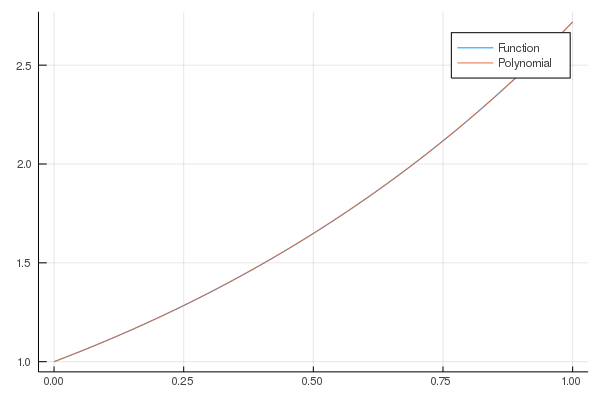
\includegraphics[width=0.55\textwidth]{1.png}}
		\caption{$n=5$}
	\end{figure}	
	\begin{figure}[!htbp]
		\centering
		{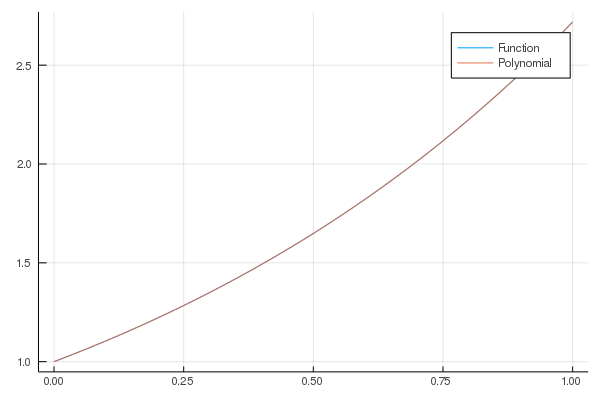
\includegraphics[width=0.55\textwidth]{2.png}}
		\caption{$n=10$}
	\end{figure}		
	\begin{figure}[!htbp]
		\centering
		{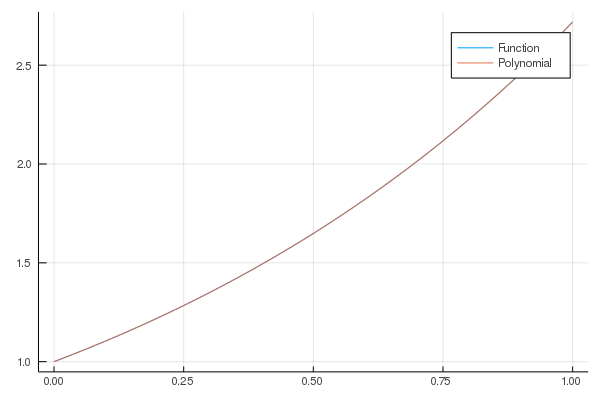
\includegraphics[width=0.55\textwidth]{3.png}}
		\caption{$n=15$}
	\end{figure}	

	\begin{figure}[!htbp]
		\centering
		{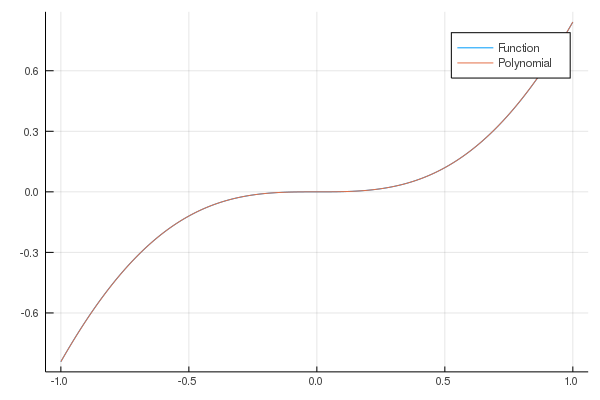
\includegraphics[width=0.55\textwidth]{4.png}}
		\caption{$n=5$}
	\end{figure}	
	\begin{figure}[!htbp]
		\centering
		{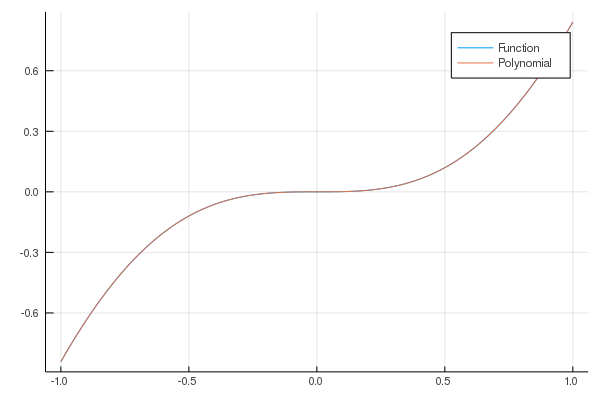
\includegraphics[width=0.55\textwidth]{5.png}}
		\caption{$n=10$}
	\end{figure}		
	\begin{figure}[!htbp]
		\centering
		{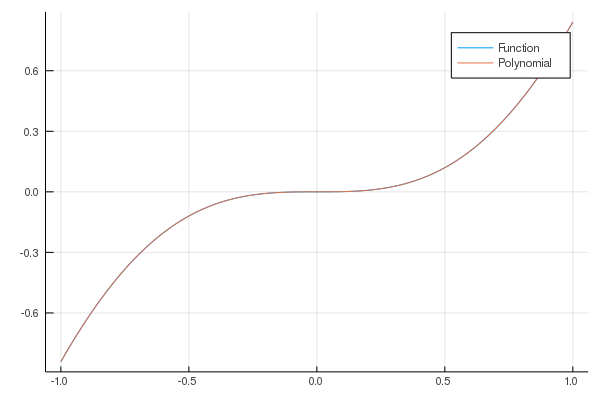
\includegraphics[width=0.55\textwidth]{6.png}}
		\caption{$n=15$}
	\end{figure}
	
\subsection{Wnioski}
Możemy zauważyć, że dla obu rozpatrywanych funkcji, wielomiany pokrywają się z interpolowaną funkcją. Im wyższy stopień wielomianu, tym wyższa dokładność, ale już dla $n=5$, wartości różnią się dopiero na szóstym miejscu po przecinku. Dla wyższych $n$ są to jeszcze bardziej odległe miejsca. 


\section{Zadanie 6}
Przetestujmy funkcje z zadania czwartego dla następujących przypadków:
\begin{enumerate}[a)]
\item $|x|, [-1, 1], n=5, 10, 15,$
\item $\frac{1}{1+x^2}, [-5, 5], n=5, 10, 15$.
\end{enumerate}

\subsection{Wyniki}
Poniższe wykresy prezentują otrzymane wyniki
	\begin{figure}[!htbp]
		\centering
		{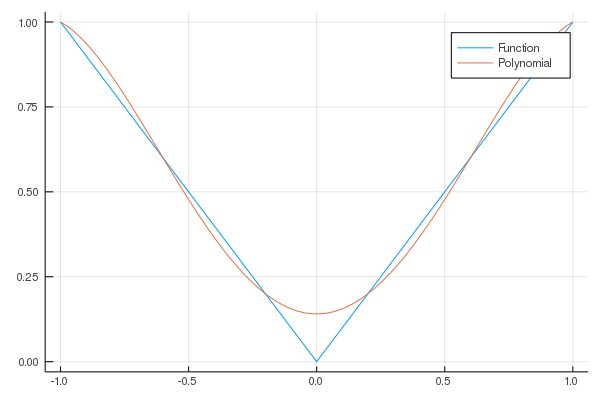
\includegraphics[width=0.55\textwidth]{7.png}}
		\caption{$n=5$}
	\end{figure}	
	\begin{figure}[!htbp]
		\centering
		{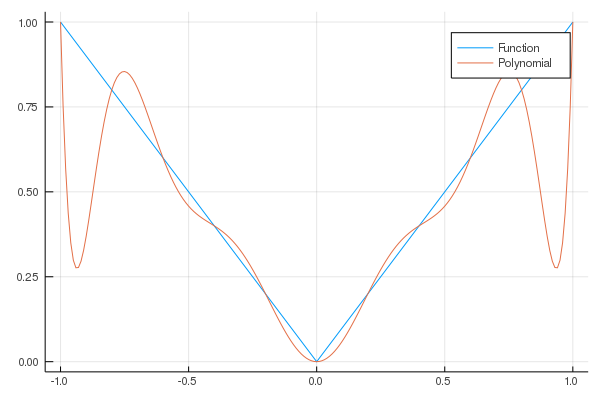
\includegraphics[width=0.55\textwidth]{8.png}}
		\caption{$n=10$}
	\end{figure}		
	\begin{figure}[!htbp]
		\centering
		{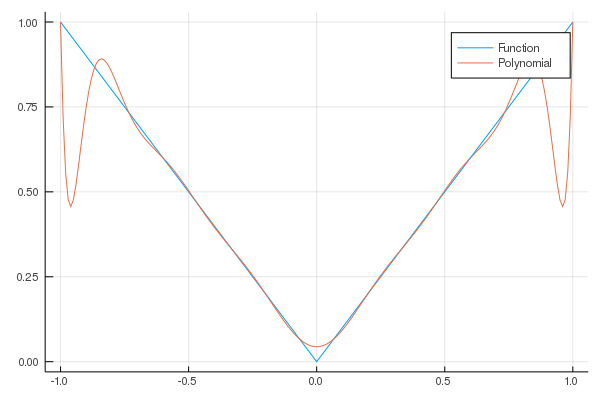
\includegraphics[width=0.55\textwidth]{9.png}}
		\caption{$n=15$}
	\end{figure}
	
	\begin{figure}[!htbp]
		\centering
		{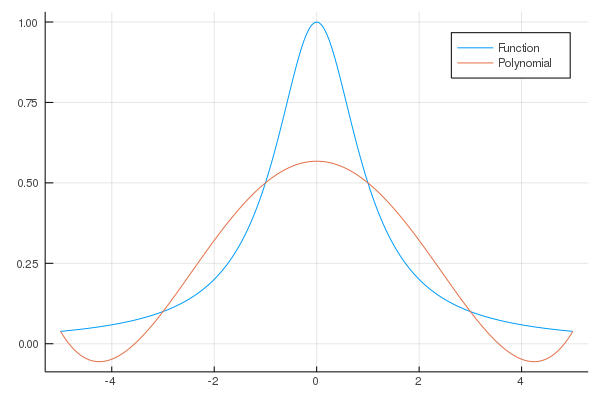
\includegraphics[width=0.55\textwidth]{10.png}}
		\caption{$n=5$}
	\end{figure}	
	\begin{figure}[!htbp]
		\centering
		{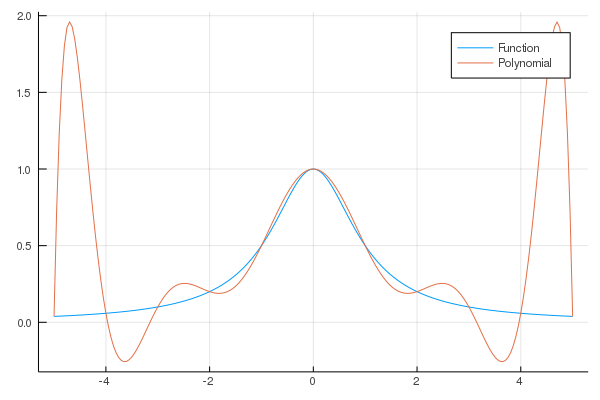
\includegraphics[width=0.55\textwidth]{11.png}}
		\caption{$n=10$}
	\end{figure}		
	\begin{figure}[!htbp]
		\centering
		{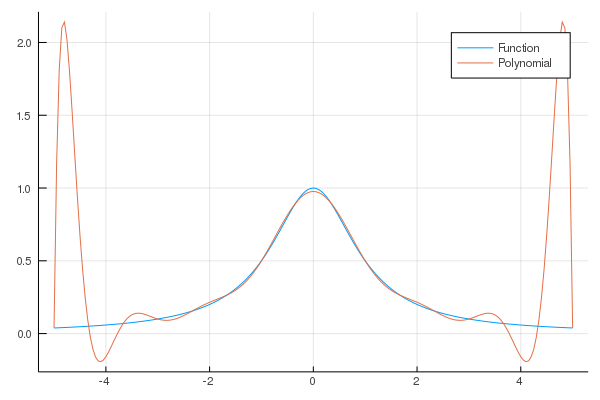
\includegraphics[width=0.55\textwidth]{12.png}}
		\caption{$n=15$}
	\end{figure}
		
\subsection{Wnioski}
W tym przypadku widać wyraźne rozbieżności, szczególnie na krańcach przedziałów. Pierwsza funkcja nie jest różniczkowalna, z tego powodu można zaobserwować odchylenie wielomianu od funkcji. Bardziej interesująca jest jednak druga funkcja, dla której od n równego około 10, zachodzi zjawisko Runge'go, co oznacza, że pomimo zwiększania ilości węzłów, dokładność interpolacji wielomianowej spada. Zjawisko to występuje czasem, kiedy odległość między kolejnymi węzłami jest stałą. Sposobem na uniknięcie tego zjawiska jest zastosowanie zmiennej odległości między węzłami. Jako węzły można również wybrać zera wielomianu Czebyszewa.
\end{document}

